\documentclass[../EBEXPaper2.tex]{subfiles}
\begin{document}
%------------------------------------------------- 
\subsubsection{Dark Measurements}
\label{sec:dark_measurements}


% Described elsewhere
%Each was connected to a 24~$\mu$H inductor and a capacitor ranging from 0.9 to 30~nF. Together they formed a bandpass filter specifying the unique bias frequency of this channel between 200 and 1200~kHz.
%The \ac{LC} board was connected to a test \ac{SQUID} board through the custom superconducting stripline described in section \ref{sec:wiring_and_RF}. The \ac{SQUID} board was mounted at the 4~K stage of a three stage either liquid helium or pulsed tube cooled test cryostat.  
%The wafer and \ac{LC} board were cooled to 250~mK by a combination of an either liquid helium or a pulse tube cooler and a three stage \heten{} sorption fridge similar to the one described in section \ref{cryogenics_and_refrigerators}.%The \ac{SQUID} board is cooled to between 4 and 5~K by the liquid helium or pulse tube cooler alone. 

For the detector dark characterization measurements, we mount the silicon device wafer, Section~\ref{sec:focal_plane_layout}, couple it to the readout electronics, Section~\ref{sec:detector_readout}, and cool it to 250-320~mK, where the exact temperature depends on the testbed. 
The measurements take place in a test cryostat or in the \ac{EBEX} cryostat itself, closed to light for characterization runs. %too specific? just say in a cryostat dedicating to testing or ebex itself?

The first test performed cold is called a network analysis. 
The network analysis sweeps a voltage across the comb in frequency and measures the current response of the circuit. 
It is a multiplexed RLC circuit with a peak in current at each LC resonant frequency, Fig.~\ref{fig:network_analysis}. 
Around 800~mK, when the niobium leads and aluminum wirebonds are superconducting but the TES is still normal, fitting the peak to a model of the multiplexed circuit gives the resonant frequencies as well as the normal resistances of the TES \citep{MacDermid_thesis}. 
%\comred{be more specific about 'the width of the peak gives.' mention this measurement ($\times$ requested fraction of $R_n$) will go into the Johnson noise?}


\begin{figure}[htbp]
\begin{center}
\epsscale{1.0}
\plottwo{images/detectors_and_readout/netanal_b16_SqCh1_5K_20111005_all.png}{images/detectors_and_readout/netanal_zoom_b16_SqCh1_5K_20111005.png}
\caption{Left: an example network analysis taken during testing.
Right: a zoom on one peak (black dots) with the fitted response (red) and the optimal bias frequency (green star) minimizing crosstalk.}
\label{fig:network_analysis}
\end{center}
\end{figure}

%The determination of the optimal bias frequency was achieved by modeling the impedance of any single branch of the multiplexed module as,
%\begin{equation}
%Z_{CLR_{i}} = R_{n_{i}} + j 2 \pi f L\left( 1- \left(f_{o_{i}} \over f \right)^{2} \right),
%\end{equation}
%where $R_{n_{i}} $ is the resistance of the bolometer, $f$ is the frequency of the voltage at each step of the network analysis, $L$ is the known value of the inductor and $f_{o_{i}} = {1 \over \sqrt{LC_{i}}}$ is the resonant frequency of the bolometer branch.
%Two additional parameters are added to account for leakage through other neighboring branches, one modeled as an inductor and the other as a capacitor.
% The current through the $i$th bolometer branch is therefore defined as,
%\begin{equation}
%I_{i} = V_{b} \left| {1 \over j 2 \pi L_{leak_i}} + {1 \over Z_{CLR_{i}}} + j 2 \pi f C_{leak_i} \right|,
%\end{equation}
%where $L_{leak_{i}}$ is a fit parameter for all other bolometer branches at lower frequency treated as a single fixed inductance and $C_{leak_{i}}$ the same for bolometer branches at higher frequencies, treated as a single capacitance.
%The final model fits over four parameters, $R_{n_{i}}$, $C_{i}$, $L_{leak_{i}}$ and $C_{leak_{i}}$.
%Though simplified somewhat, this model fits the data quite well, as can be seen in Fig.~\ref{fig:bolometer_comb_fit}.
%It should be noted that the final bias frequency for a single branch is not the peak of the current, but rather the calculation of $f_{o_{i}}$ given the $C_{i}$ from the fit.
%This ensures that the carrier frequency is selected to maximize current through this branch, not through the circuit as a whole, as the latter would increase crosstalk.


Histograms summarizing the measured normal resistance values for the three \ac{EBEX} frequency bands are shown in Fig.~\ref{fig:rn_histograms}. 
The target normal resistance for all bands is 1.5~$\Omega$ in order to ensure the detector remains in the stable regime where the detector electrical bandwidth, determined in part by the resistance, appropriately exceeds the \ac{TES} thermal bandwidth. 
%Section~\ref{sec:detector_optimization}. the optimization section doesn't actually provide the detail I want it to provide.
We find the median normal resistance, $R_{normal}$, for the 150, 250, and 410~GHz bands to be 1.9, 1.5, and 1.0~$\Omega$ respectively. 
The consequences of overshooting this value, as is the case for many of the 150~GHz detectors, are an increase in the detector voltage bias leakage, which is proportional to $R^2$ \citep{dobbs_revSciInst_2012}, and a decrease in the loopgain, which is inversely proportional to R. 
% if R is higher, then johnson current noise is decreased since it goes like 1/sqrt(R)
% if R is higher, then stability requirement has R/(2*pi*L) > 5.8/tau_tes is more satisfied
For a detector dropped to 85\% in the transition, having a normal resistance of 1.9~$\Omega$ instead of 1.5~$\Omega$ results in a bias leakage increase of 60\%, increasing the cross-talk from 0.5\% to 0.8\%, and a loopgain decrease of 30\%. 
The consequence of undershooting the normal resistance, as is the case for many of the detectors on wafer 410-28, is an increase in the Johnson current noise. The Johnson noise is proportional to $1/\sqrt{R}$, so that noise term increases by 20\% given a value of 1.0~$\Omega$ instead of 1.5~$\Omega$.

%\comred{Assume detector optimization explains what about the electronics set our target to be 1.5~$\Omega$? Ben says "The requirement is really ~1.25 because what actually matters is Rtes in transition for the L/R requirement.  So depending on how deep we get in to the transition we could start anywhere just above 1.2 Ohms to operate at 0.88 to 1.0 Ohms." BUT. When determining which Rfrac to tune to, we didn't do this calculation. Rather, we noted, in general, below 80\% $R_{start}$, we had (not well understood) excess noise and so opted to go to 85\%. What I'm trying to say is, in practice, the operating fracRn value was not chosen carefully on a bolo by bolo basis or even a wafer by wafer basis to achieve a specific L/R. Explain the consequence of having a higher or lower normal resistance, e.g. 150s and one of the 410s (was it the 410 that operated or the 410 that was saturated?)? Ben says "Increased johnson noise and possibly bolo stability.  However, I'm not sure if either of these effects were detected in the wafers in test cryostats, Palestine, or flight."}


\begin{figure}[ht!]
\centering
\subfigure[150 GHz]
{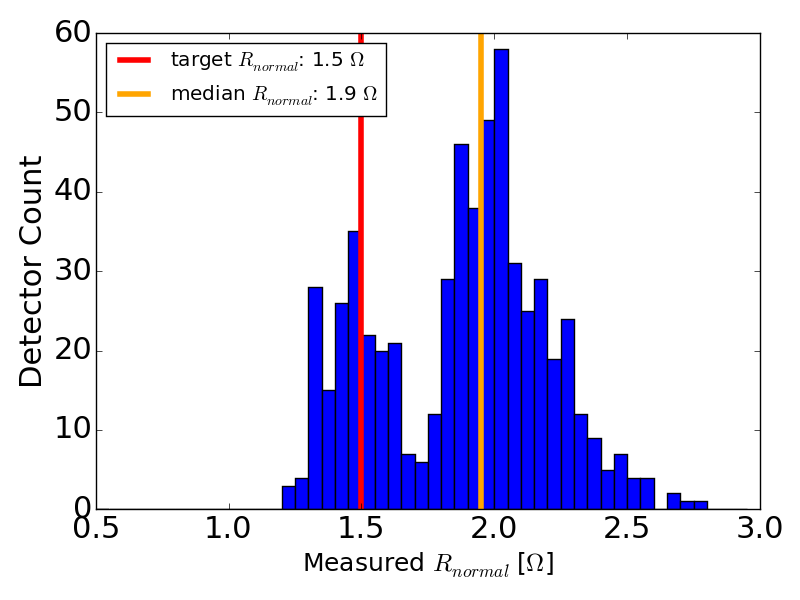
\includegraphics[width=0.31\textwidth]{./images/150_rn_hist}\label{subfig:150 GHz rns}}
\subfigure[250 GHz]
{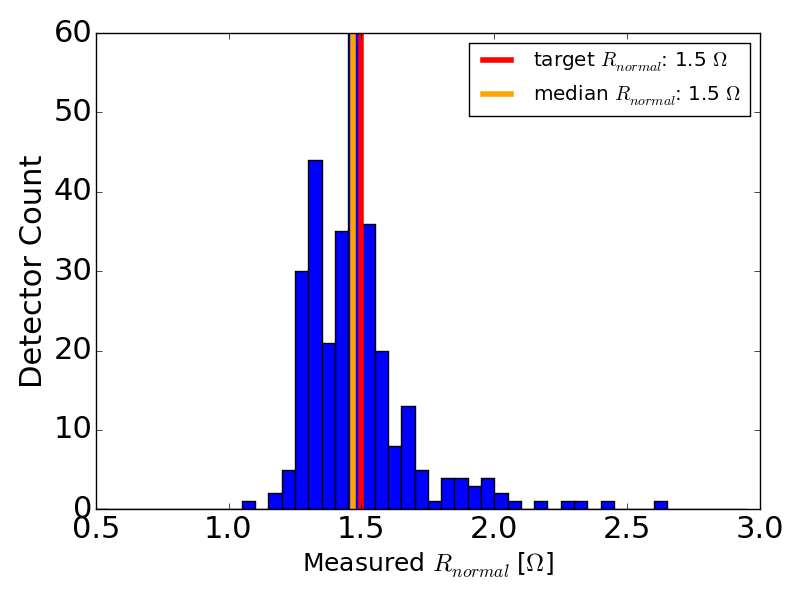
\includegraphics[width=0.31\textwidth]{./images/250_rn_hist}\label{subfig:250 GHz rns}}
\subfigure[410 GHz]
{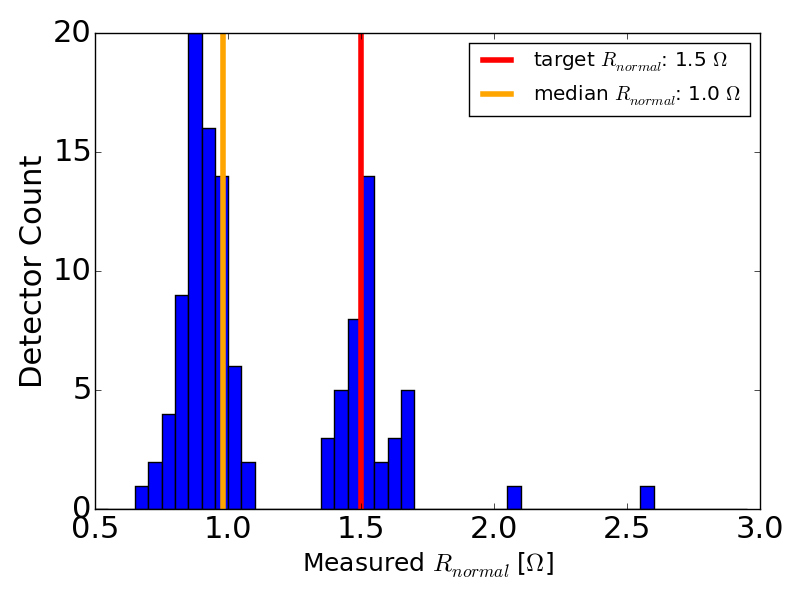
\includegraphics[width=0.31\textwidth]{./images/410_rn_hist}\label{410 GHz rns}}
\caption{\textbf{From Left to Right:} Histogram of the measured normal resistance, $R_{normal}$, values for the 150, 250, and 410~GHz band \ac{EBEX} detectors operated during the \ac{EBEX2013} ballon flight. The design target for each frequency band, 1.5~$\Omega$, is the vertical red line and the median measured normal resistance is the vertical gold line.}
\label{fig:rn_histograms}
\end{figure}

Once the resonant frequencies are determined from the network analysis fits, the stage is heated so the bolometers are above their critical temperatures. 
The bolometers are then electrically overbiased such that there is enough Joule Power dissipated in the \ac{TES} to keep its resistance normal as the stage is cooled. 
Once the stage is at its base temperature, we measure the bolometer saturation powers. 
The saturation power is an important indicator of bolometer sensitivity on the sky because the sensitivity of the bolometer increases with lower saturation power, but the bolometer loses nearly all sensitivity if it saturates, i.e. its saturation power is less than the optical load during observations. 
%measure the average thermal conductances, $\overline{G}$, via performing IV curves. 
In order to measure the saturation power, we perform IV curves. 
That is, for each biased channel, we step down the voltage bias, typically in steps of 0.05~$\mu V$, and measure the current through the bolometer. 
%As the Joule Power decreases, the detector temperature decreases towards its transition temperature and the . 
Each channel is dropped until it reaches a fixed fraction of its original resistance, typically 85\%.
In the case of a well-behaved bolometer with small stray impedance, electro-thermal feedback causes the power at the bolometer to remain fixed once the bolometer is sufficiently far into transition \cite{lanting_thesis}.
Each bolometer wafer is enclosed in a light-tight box for these tests, so the total electrical power supplied is equivalent to the saturation power. 
An example of the IV, PV, RV curves is shown in Fig.~\ref{fig:bolo_iv_curve}, where the saturation power is the horizontal section of the PV curve.

\begin{figure}[htbp]
\begin{center}
\epsscale{0.8}
\plotone{images/detectors_and_readout/IV_curve} 
\caption{The current (top panel), power (middle panel) and resistance (bottom panel) of a bolometer channel versus the electrical bias on the detector. The bolometer can be seen to drop into transition with a saturation power of about 9~pW. \acomment{Will likely want to replace this with non-scaled version}  \comgreen{Franky has the data and the code to produce this plot.} \comred{what does non-scaled version mean? do we want r vs v since we don't use or talk about it? or should we point out more explicitly this is how the fraction of Rn is determined??}}
\label{fig:bolo_iv_curve}
\end{center}
\end{figure}

%Will probably be able to cut most of this.

%The first step in the saturation power measurement to overbias the detectors. 
%That is, sufficient electrical power needed to be applied to each bolometer to avoid them latching superconducting when cooled to their 250-300~mK operating temperatures.
%In some cases channels would have much higher thermal conductances than expected, resulting in channels that latched superconducting when the wafer was cooled.
%This was detected as a sharp transition in the mean value of the timestream and an increase in noise by a factor of 5-10 for this channel, and often other channels on this multiplexed module.
%Some of these channels were recovered for the dark tests by rewarming the wafer and pproviding a much higher electrical bias.
%For others no suitable electrical bias could be found and they were left unbiased to permit testing of the rest of the channels on that multiplexed module.
%In the latter case the channels were electrically disconnected before the wafer was installed the \ac{EBEX} receiver.

%The measurement of the saturation power was performed by decreasing the electrical power on every bolometer on the same multiplexed module in steps.
%At each step the DfMUX board used digital active nulling (DAN) to null the current at the \ac{SQUID} coil at 12~kHz \cite{deHann_DAN2012}. 
%The bias on all channels on the same module were dropped simultaneously to attempt to minimize the effect of bolometer to bolometer bias leakage, wherein the electrical bias from a single channel leaks slightly into its neighbours in frequency space.

%In practice, the saturation powers for bolometer channels were often measured twice, as the overbias electrical biases were typically much higher than necessary for the first measurement. 
%This exacerbated the bolometer bias leakage, as well as causing some bolometers not to drop sufficiently into transition, if the slope of the RV curve above the transition was steep enough.
%The second set of measurements were performed after manually adjusting each bolometer electrical bias to be just above the region with significant change in slope of the resistance-voltage curve. 
%The number of detectors which successfully entered transition in the second set of saturation power measurements was often higher by 5 to 10\%, and the saturation powers would vary by less than 0.5~pW. %Should probably double check these numbers.

%The saturation power alone is not sufficient to understand the on-sky performance of a bolometer.
%Measurement of the thermal conductance is also required. 
%This, in turn, requires a measurement of the critical temperature of the bolometer. 

%In order to understand the on-sky performance of the bolometers, 
We also need to measure the detectors' critical transition temperatures from normal resistivity to superconductivity. 
The phonon and Johnson noise terms are a function of the critical temperature,  Section~\ref{sec:noise_performance}, and the detector thermal conductance is also a function of the critical temperature. 
For the measurement of the critical temperature, we place a tiny voltage bias of 5~$nV_{rms}$ across the detector such that the Joule heating is negligible ($\frac{V^2}{R} = 1.5~fW$) but there is still a measurable current signal. 
Then we slowly, usually less than 3~mK/min, cool and warm the detectors through their transitions while measuring the current through the detector. We convert to resistance using Ohm's law, $R=V_{bias}/I_{measured}$.

Fig.~\ref{fig:tc_measurement} is an example of a critical temperature measurement for one detector. 
The top panel shows the detector temperature as a function of time. %no need to point out there is hysteresis inherent in this measurement because the temperature sensor is on the invar, not on the wafer? 
The bottom two panels show the bolometer resistance as a function of time and temperature. 
The hysteresis between the critical temperature measured cooling and warming is generally less than 5~mK, sufficiently accurate for characterization.

\begin{figure}[htbp]
\begin{center}
\epsscale{0.6}
\plotone{images/detectors_and_readout/410-18-03-03_tc}
\caption{The critical temperature of bolometer 410-18-03-03 is 450~mK.  The temperature as a function of time (top panel), resistance as a function of time (middle panel) and temperature as a function of resistance (bottom panel) curves used to determine the critical temperature are shown. \comred{bottom panel has axis labels switched! where is the data/code to reproduce this plot?}
}
\label{fig:tc_measurement}
\end{center}
\end{figure} 

Histograms summarizing the measured critical temperatures for the three \ac{EBEX} frequency bands are shown in Fig.~\ref{fig:tc_histograms}. 
The target critical temperature for each band is 0.44~K, a value which optimizes the phonon noise term given the \ac{EBEX} bath temperature. %or refer to Section~\ref{sec:detector_optimization} for the motivation ??
We find the median critical temperature for the 150, 250, and 410 GHz bands to be 0.45, 0.49, and 0.51~K respectively.  
The consequence of overshooting the critical temperature, as for some of the detectors in each of the frequency bands, is an increase in the Johnson noise, proportional to $\sqrt{T}$, and an increase in the phonon noise, proportional to $T$. 
The consequence of undershooting the critical temperature, as for roughly half of the 150~GHz detectors, is potentially not being able to drop the detector into the transition because the critical temperature is too close to the bath temperature. % is this actually why we didn't want to go too low?
%\comred{what's the consequence of the wide spread in Tc for the 150s? how concerned are we about the level of spread we fabricated?}

\begin{figure}[ht!]
\centering
\subfigure[150 GHz]
{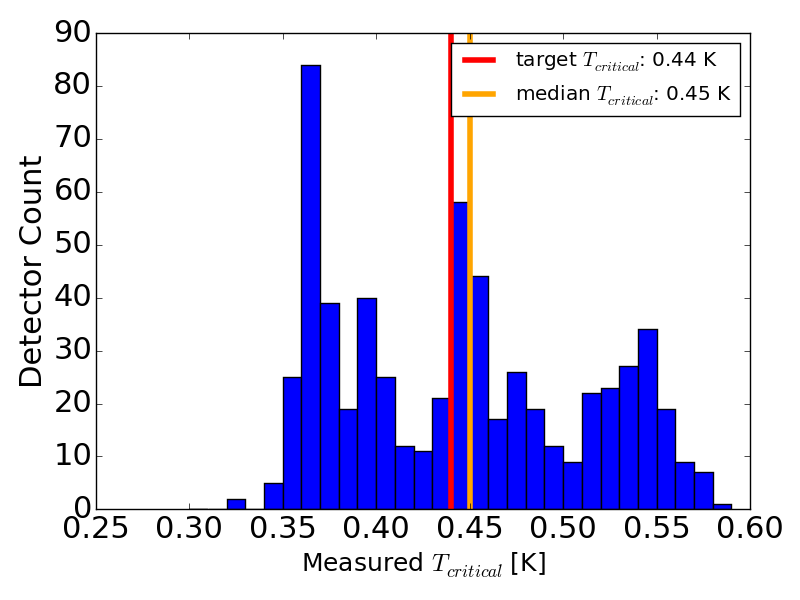
\includegraphics[width=0.31\textwidth]{./images/150_tc_hist}\label{subfig:150 GHz tcs}}
\subfigure[250 GHz]
{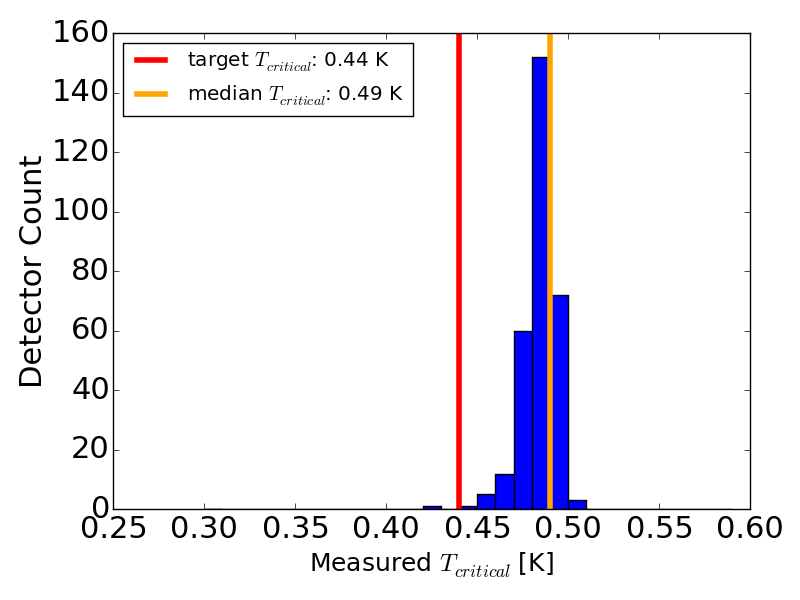
\includegraphics[width=0.31\textwidth]{./images/250_tc_hist}\label{subfig:250 GHz tcs}}
\subfigure[410 GHz]
{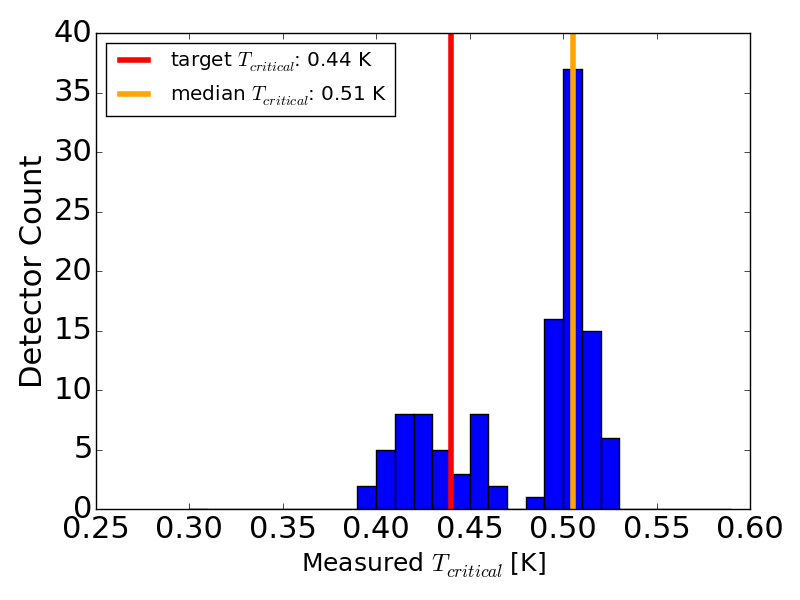
\includegraphics[width=0.31\textwidth]{./images/410_tc_hist}\label{410 GHz tcs}}
\caption{\textbf{From Left to Right:} Histogram of the measured critical temperature, $T_{critical}$, values for the 150, 250, and 410~GHz band \ac{EBEX} detectors operated during the \ac{EBEX2013} ballon flight. The design target for each frequency band, 0.44~K, is the vertical red line and the median measured critical temperature is the vertical gold line. \comred{was it one of the 250s that had no tc measurements and so we used the average/median value of 490? and so there are too many detectors in the 250 histogram?}}
\label{fig:tc_histograms}
\end{figure}

Once we have measured the saturation powers and critical temperatures, then we can find the average thermal conductance of each detector via $\overline{G} = P_{sat}/\Delta T$, where $\Delta T$ is the difference between the critical and bath temperatures, $T_{critical} - T_{bath}$. 
We need the thermal conductances in addition to the saturation powers in order to predict the phonon noise contribution. 
Histograms summarizing the measured average thermal conductance values for the three \ac{EBEX} frequency bands are shown in Fig.~\ref{fig:G_Histograms}, where we find the median average thermal conductance, $\overline{G}$, for the 150, 250, and 410 GHz bands to be 36, 51, and 69~pW/K respectively. 
The target values for the average thermal conductances are set by the radiative loading in the balloon environment, Section~\ref{sec:detector_optimization}, and are 30, 40, and 50~$pW/K$ for the 150, 250, and 410~GHz bands respectively. 
Overshooting the average thermal conductance means an increase in the phonon noise, proportional to $\sqrt{G}$. 
The consequence of undershooting the thermal conductance is exactly as it is for undershooting the saturation power. 
That is, we risk saturation of the detector if there is not enough thermal conductance along the weak link to dump the incident power on the bolometer at float to the bath. 
The goal was thus to err on the higher side of the target. 

%36.2, 53.5, and 60.9 pW/K respectively. %where are these numbers from ??
%\comred{You don't say why we care about G. What about the targets? And, as with the other dark measurements, what's the consequence of having this particular set of measured $\overline{G}$s?}

\begin{figure}[ht!]
\centering
\subfigure[150 GHz]
{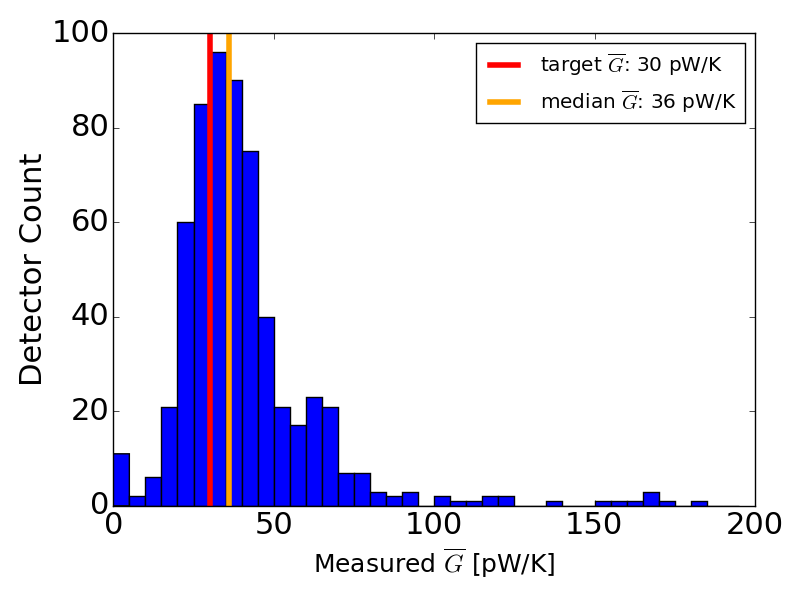
\includegraphics[width=0.31\textwidth]{./images/150_g_bar_hist}\label{subfig:150 GHz Gs}}
\subfigure[250 GHz]
{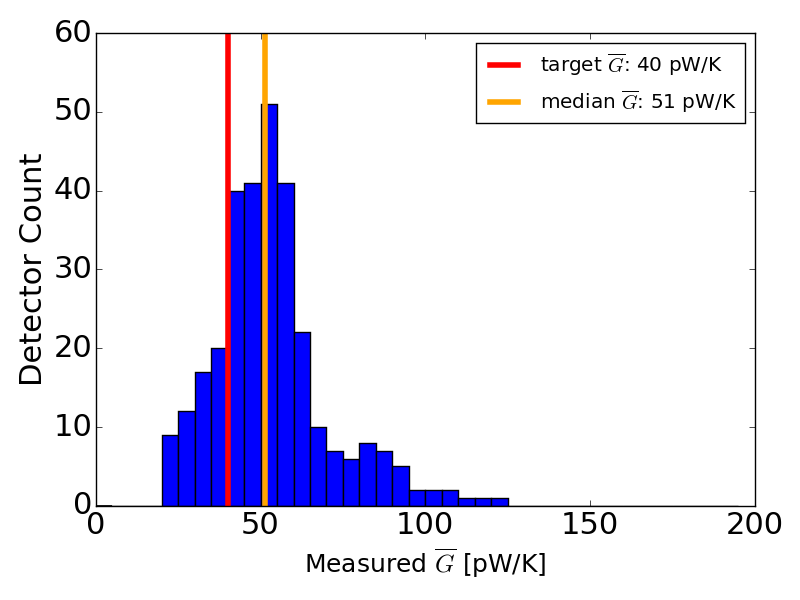
\includegraphics[width=0.31\textwidth]{./images/250_g_bar_hist}\label{subfig:250 GHz Gs}}
\subfigure[410 GHz]
{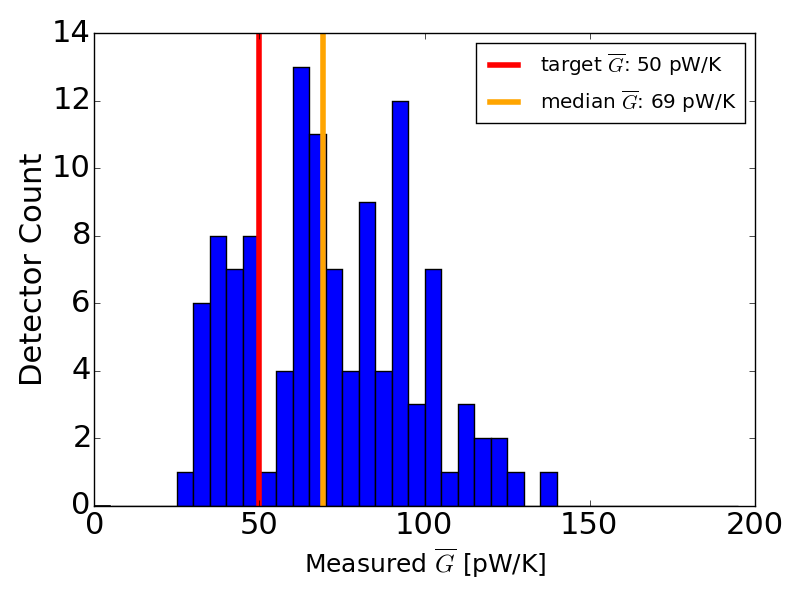
\includegraphics[width=0.31\textwidth]{./images/410_g_bar_hist}\label{410 GHz Gs}}
\caption{\textbf{From Left to Right:} Histogram of the measured average thermal conductance, $\overline{G}$, values for the 150, 250, and 410~GHz band \ac{EBEX} detectors operated during the \ac{EBEX2013} ballon flight. The design target for each frequency band is the vertical red line and the median measured average thermal conductance is the vertical gold line. \comred{ben's (or who made them?) 410 histogram had a much prettier distribution/cutoff... are we using different data somehow?? since 410-18 didn't actually work during flight, should I exclude those guys?}}
\label{fig:G_Histograms}
\end{figure}



%\comred{I think you've used base and bath and stage temperatures interchangeably. pick just one??}




%------------------------------------------------
%\include{DetectorReadoutBibliography}
\end{document}